\documentclass[11pt, oneside]{article} 	% use "amsart" instead of "article" for AMSLaTeX format
\usepackage{geometry} 		% See geometry.pdf to learn the layout options. There are lots.
\geometry{letterpaper}  		% ... or a4paper or a5paper or ... 
\usepackage[parfill]{parskip} 		% Activate to begin paragraphs with an empty line rather than an indent
\usepackage{graphicx}				% Use pdf, png, jpg, or eps§ with pdflatex; use eps in DVI mode
								% TeX will automatically convert eps --> pdf in pdflatex		
\usepackage{amssymb}
\usepackage{amsmath}
\usepackage{authblk}
\usepackage[
backend=biber,
style=alphabetic,
]{biblatex}
\usepackage{graphicx}
\graphicspath{ {./images/} }
\usepackage{verbatim}
\usepackage{tikz} 
\usepackage{subfig}

\usepackage{syntonly}

% \syntaxonly \langle -- use this for checking syntax only
% \mbox {text} - keep together
% \fbox {text} - keep together and draw around

%\pagestyle{plain|headings|empty} % header and footer p.27
%SetFonts
%\include{filename}, \includeonly{filename1, filename2} , \input[fiename}

%SetFonts% 


\title{Polynomial Uniqueness by way Graph Tournament Graphs}
\author{Dave Fetterman}
\affil{Obviously Unemployed}
\date{2/10/23}
\begin{document}
\maketitle

\begin{abstract}

TODO\cite{1}

\end{abstract}


\section{Pieceyard}

% Graph drawing reference: https://www.baeldung.com/cs/latex-drawing-graphs
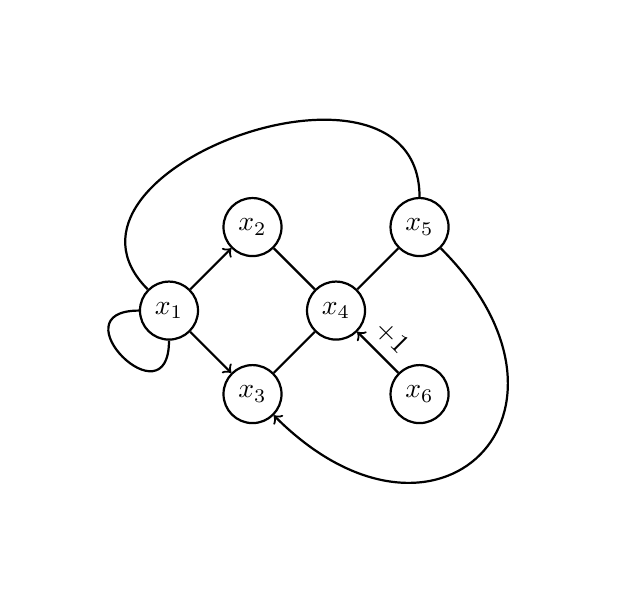
\begin{tikzpicture}[node distance={15mm}, thick, main/.style = {draw, circle}] 
\node[main] (1) {$x_1$}; 
\node[main] (2) [above right of=1] {$x_2$}; 
\node[main] (3) [below right of=1] {$x_3$}; 
\node[main] (4) [above right of=3] {$x_4$}; 
\node[main] (5) [above right of=4] {$x_5$}; 
\node[main] (6) [below right of=4] {$x_6$}; 
\draw[->] (1) -- (2); 
\draw[->] (1) -- (3); 
\draw (1) to [out=135,in=90,looseness=1.5] (5); 
\draw (1) to [out=180,in=270,looseness=5] (1); 
\draw (2) -- (4); 
\draw (3) -- (4); 
\draw (5) -- (4); 
\draw[->] (5) to [out=315, in=315, looseness=2.5] (3); 
\draw[->] (6) -- node[midway, above right, sloped, pos=1] {+1} (4); 
\end{tikzpicture} 


 $\det\begin{bmatrix}
1 & a & a^2 & \ldots & a^{n-1} \\
1 & b & b^2 & \ldots & b^{n-1} \\
\vdots & & & & \vdots  \\
1 & x & x^2 & \ldots & x^{n-1} \\
\end{bmatrix} \cdot \hat{n}$



\begin{center}
\begin{tabular}{||c c c c||} 
 \hline
 Col1 & Col2 & Col2 & Col3 \\ [0.5ex] 
 \hline\hline
 1 & 6 & 87837 & 787 \\ 
 \hline
 2 & 7 & 78 & 5415 \\
 \hline
 3 & 545 & 778 & 7507 \\
 \hline
 4 & 545 & 18744 & 7560 \\
 \hline
 5 & 88 & 788 & 6344 \\ [1ex] 
 \hline
\end{tabular}
\end{center}


\section{TODO}
\subsection{TODO}

\begin{thebibliography}{9}
\bibitem{1}
Wikipedia: \url{https://en.wikipedia.org/wiki/Vandermonde_matrix}
\end{thebibliography}


\end{document}

